\documentclass[10pt,journal]{IEEEtran}
%\IEEEoverridecommandlockouts

\usepackage[utf8]{inputenc}
\usepackage[spanish,es-tabla]{babel} % Idioma español con tablas
\usepackage[spanish]{babel}
\usepackage[table,xcdraw]{xcolor} % Para pintar tablas
\usepackage{url} % Para colocar URL
\usepackage{amsmath,amssymb,amsfonts}
\usepackage{graphicx}
\usepackage{textcomp}
\usepackage{xcolor}
\usepackage{float} % Para var H, figure

\usepackage[square,numbers]{natbib}
\bibliographystyle{abbrvnat}

\renewcommand{\baselinestretch}{1.59}     %interlineado

\title{Uso de las listas enlazadas (punteros) en Archivos y Base de Datos}

\author{
\IEEEauthorblockN{{\Large Angely Mendez Cruz}} \\
\vspace{2mm}
\IEEEauthorblockA{\textit{Organización de Archivos} \\
\textit{Escuela de Informática} \\
\textit{Facultad de Ciencias Físicas y Matemáticas} \\
\textit{Universidad Nacional de Trujillo, \\ Perú }
\\ \vspace{1mm}
t052701020@unitru.edu.pe}}

\begin{document}

\maketitle

    \begin{abstract}
    En este trabajo de investigación se brinda información, respecto al uso de las listas enlazadas (punteros), considerada también como una estructura ligada, que almacena una colección de elementos generalmente llamados nodos, en donde cada nodo puede almacenar datos y ligas a otros, estos nodos poseen dos campos uno para almacenar la información o valor del elemento y otro para el enlace que determina la posición del siguiente elemento o nodo de la lista, por lo que sus usos están vinculados directamente a la optimización de archivos y a las colas, con el método FIFO en las órdenes de compra y atención en los productos.
    \end{abstract}
    
    \section{\textbf{Introducción}}
    
    En la actualidad y ante la evolución de las estructuras de datos, siendo esta una forma particular de organizar datos en un computador para que puedan ser utilizados de manera eficiente, generalmente son la clave para diseñar algoritmos eficientes. Un claro ejemplo de ellas son las listas vinculadas o enlazadas dinámicas, cuyo tamaño de lista puede cambiar en tiempo de ejecución, por ejemplo se puede imaginar una lista enlazada como una cadena donde cada enlace está conectado al siguiente para formar una secuencia con un comienzo y un final y donde sus usos se relacionan a los sistema de  archivos.
    
    \section{\textbf{Listas Enlazadas (punteros)}}
    \subsection{\textbf{Definición}}
    Una \textbf{lista vinculada o enlazada}, es un conjunto de nodos asignados dinámicamente, organizados de tal manera que cada nodo contiene un valor y 
    un puntero \cite{Listasvi9:online}. Por lo que el puntero siempre apunta al siguiente miembro de la lista. Si el puntero es NULL, entonces es el último nodo de la lista.

    Una lista vinculada se mantiene utilizando una \textit{variable de puntero local} que apunta al primer elemento de la lista. Si ese puntero también es NULL, se considera que la \textbf{lista está vacía}, (ver Figura  ~\ref{f11}).
    
    \begin{figure}[H]
        \begin{center}
        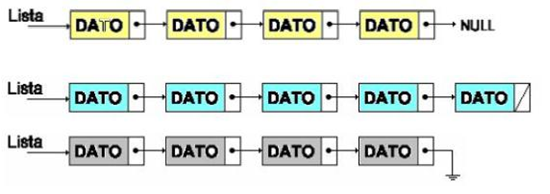
\includegraphics[width=7.5cm, height=4cm]{Imagenes/Lista.png}
        \caption{Representación de un lista enlazada}
        \label{f11} 
        \end{center}
    \end{figure}
    
    Además, es considerada una de las \textbf{estructuras de datos básicas en computación}, aunque tal vez no tan conocida. Hace tiempo, el profesor David Brailsford de la universidad de Nottingham explicó en un video en Computerphile cómo funcionan las listas enlazadas \cite{Punteros25:online}. El profesor usa bloques de Lego para comunicar de manera simple las ideas detrás de esto.
    
    La Universidad de Sevilla en España, dentro de sus Fundamentos de Informática definen a las listas enlazadas como una estructura de datos lineal, ver Figura  ~\ref{f22} formada por \textbf{bloques de información} \cite{Microsof65:online}, con un formato común, enlazados entre sí mediante punteros.
    
    \begin{figure}[H]
        \begin{center}
        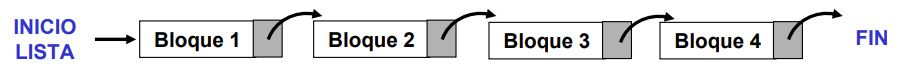
\includegraphics[width=9cm, height=1.8cm]{Imagenes/Lista2.JPG}
        \caption{Lista enlazada - Universidad de Sevilla}
        \label{f22} 
        \end{center}
    \end{figure}
    
    \subsection{\textbf{Características}}
    Dado que las listas enlazadas son una estructura lineal que almacena una colección de elementos generalmente llamados nodos, en donde cada nodo puede almacenar datos y ligas a otros nodos.
    
    Tienen estructuras dinámicas que se utilizan para almacenar datos que están cambiando constantemente y cuentan con algunas principales características \cite{george1999introduccion} dentro de estas, las que resaltan son:
    \begin{itemize}
    \item \textbf{Los elementos se distribuyen de forma dispersa por la memoria:}
    Los bloques de información no ocupan posiciones consecutivas en la memoria. El orden de la lista la establecen los enlaces entre bloques de información.
    \item \textbf{Acceso a los elementos aleatorio:}
    Puede extraerse información de cualquier elemento o insertar un bloque en cualquier posición.
    \item \textbf{Acceso a los elementos no destructivo:}
    Al contrario que en colas y pilas, la extracción de un bloque no implica su eliminación.
    \item \textbf{El tamaño de la lista puede modificarse de forma dinámica:}
    Al contrario que en colas y pilas, no hay un número máximo de elementos de la lista (salvo limitaciones de la capacidad de almacenamiento de la máquina).
    \end{itemize}
    
    Existen diferentes \textbf{tipos de listas enlazadas:} listas enlazadas \textit{simples}, listas \textit{doblemente enlazadas}, listas enlazadas \textit{circulares} y listas enlazadas \textit{doblemente circulares}.
    
    Por otro lado, las listas enlazadas pueden ser implementadas en muchos lenguajes lo que las convierte factibles para su comprensión y posterior aplicación.
    \begin{itemize}
        \item Lenguajes tales como \textbf{Lisp, Scheme y Haskell} tienen estructuras de datos ya construidas, junto con operaciones para acceder a las listas enlazadas.
        \item Lenguajes imperativos u orientados a objetos tales como \textbf{C o C++ y Java}, respectivamente, disponen de referencias para crear listas enlazadas.
    \end{itemize}
    
    Dentro de las \textbf{operaciones más comunes} en las listas enlazadas se encuentran: \textit{crear} la lista, \textit{insertar} un elemento en la lista en determinada posición, \textit{eliminar} un elemento de la lista o toda la lista, \textit{buscar y recuperar} un elemento en la lista, recorrer la lista e imprimirla, \textit{ordenar} la lista según algún criterio, insertar un elemento en forma ordenada, preguntar si la lista está vacía, obtener la cantidad de elementos, etc.
    
    \subsection{\textbf{Diferencia entre Listas enlazadas y Arreglos}}
    Al igual que los arreglos, las listas enlazadas o por su nombre en inglés \textit{\textbf{Linked List}} son una estructura de datos lineal \cite{LinkedLi27:online}. Y a diferencia de las mencionadas inicialmente, los elementos de la lista enlazada \textbf{no se almacenan en una ubicación contigua}; los elementos están vinculados mediante punteros.
    
    Respecto a ello, las arreglos se pueden utilizar para almacenar datos lineales de tipos similares, pero las arreglos tienen las siguientes limitaciones:
    \begin{enumerate}
        \item El \textbf{tamaño de las arreglos es fijo}, por lo que debemos conocer el límite superior del número de elementos de antemano. Además, generalmente, la memoria asignada es igual al límite superior independientemente del uso. 
        \item \textbf{Insertar un nuevo elemento} en una serie de elementos es \textbf{costoso} porque debe crearse espacio para los nuevos elementos y para crearlo, los elementos existentes deben cambiarse. 
    \end{enumerate}
    
    A continuación, un cuadro comparativo, (Ver Tabla ~\ref{tab1} ) entre ellas:

    \begin{table}[H]
    \centering
    \caption{Listas Enlazadas y Arreglos}
    \label{tab1}
    \begingroup
    \setlength{\tabcolsep}{6pt} % Default value: 6pt
    \renewcommand{\arraystretch}{1.4} % Default value: 1
   \begin{tabular}{|cc|lll}
    \cline{1-2}
    \multicolumn{2}{|c|}{\cellcolor[HTML]{000000}{\color[HTML]{FFFFFF}      \begin{tabular}[c]{@{}c@{}}Diferencia entre Listas Enlazadas\\ y Arreglos\end{tabular}}}                                                                        &  &  &  \\ \cline{1-2}
    \multicolumn{1}{|c|}{\cellcolor[HTML]{C0C0C0}Listas Enlazadas}                                                             &                \cellcolor[HTML]{C0C0C0}Arreglos                                                                      &  &  &  \\ \cline{1-2}
    \multicolumn{1}{|c|}{\begin{tabular}[c]{@{}c@{}}Capacidad para insertar \\ y eliminar\\ elementos indefinido.\end{tabular}} &           \begin{tabular}[c]{@{}c@{}}Capacidad limitada en la\\ inserción, eliminación \\ necesita redimensión.\end{tabular} &  &  &  \\ \cline{1-2}
    \multicolumn{1}{|c|}{Acceso secuencial}                                                                                    & Acceso     aleatorio                                                                                      &  &  &  \\ \cline{1-2}
    \multicolumn{1}{|c|}{Tamaño Dinámico}                                                                                      & Tamaño Fijo                                                                                           &  &  &  \\ \cline{1-2}
    \end{tabular}
    \endgroup
    \end{table}
   
    \section{\textbf{Usos de las listas enlazadas (punteros) en archivos y base de datos}}
    
    \begin{enumerate}
    \item \underline{\textbf{En Archivos}} \\
    Probablemente la cuestión más importante al implementar el almacenamiento de archivos sea mantener un registro acerca de qué bloques de disco van con cuál archivo, el método más usado es la Asignación de archivos con listas enlazadas.

    Las listas enlazadas son utilizadas en el \textbf{almacenamiento de archivos} \cite{enlazada18:online}, cuya intención es mantener a cada uno como una lista enlazada de bloques de disco, como se muestra en la Figura  ~\ref{f33}.
    
     La primera palabra de cada bloque se utiliza como apuntador al siguiente. El resto del bloque es para los datos. A diferencia de la asignación contigua, en este método, se puede utilizar cada bloque del disco.
    
     \begin{figure}[H]
        \begin{center}
        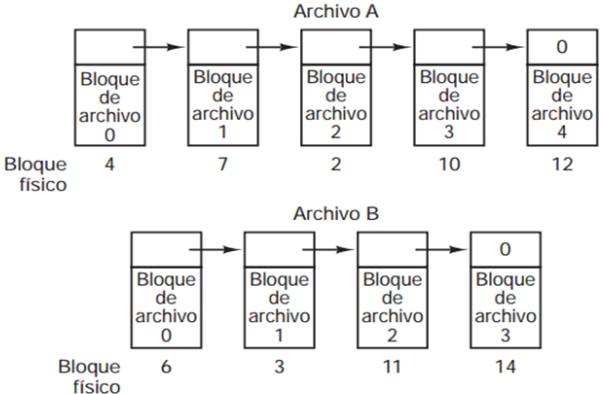
\includegraphics[width=8cm, height=5cm]{Imagenes/Archivo1.png}
        \caption{Lista enlazada}
        \label{f33} 
        \end{center}
    \end{figure}
    
    \textbf{No se pierde espacio debido a la fragmentación del disco} (excepto por la fragmentación interna en el último bloque).
    
    Además, para la entrada del directorio sólo le basta con \textbf{\textit{almacenar la dirección de disco del primer bloque}}. El resto se puede encontrar a partir de ella.

    Por otro lado, aunque la lectura secuencial en un archivo es directa, el acceso aleatorio es en extremo lento. Para llegar al bloque n, el \textbf{sistema operativo} tiene que empezar desde el principio y leer los n– 1 bloques anteriores, uno a la vez. Es claro que tantas lecturas serán demasiado lentas.
    
    Otro inconveniente viene dado por \textbf{el espacio requerido por los punteros}. Una solución a este problema consiste en no asignar bloques individuales, sino conjuntos de bloques denominados clusters. De esta forma el porcentaje de espacio perdido por los punteros se reduce. 
    
    Además, la cantidad de \textbf{almacenamiento de datos} en un bloque ya no es una potencia de dos, debido a que el apuntador ocupa unos cuantos bytes.
    
    Aunque no es malo, tener un tamaño peculiar es menos eficiente debido a que muchos programas leen y escriben en bloques, cuyo tamaño es una potencia de dos.
    
    Con los primeros bytes de cada bloque ocupados por un apuntador al siguiente bloque, \textbf{leer el tamaño del bloque completo} requiere \underline{adquirir y concatenar información} de dos bloques de disco, lo cual genera un gasto adicional de procesamiento debido a la copia, ver Figura ~\ref{f44}.
    
    \begin{figure}[H]
        \begin{center}
        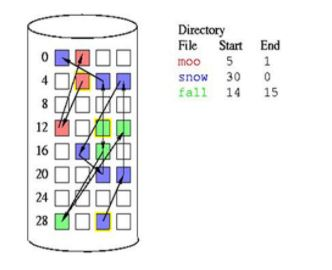
\includegraphics[width=8.4cm, height=5cm]{Imagenes/Archivo2.JPG}
        \caption{Asignación por Lista Enlazada - Linked Allocation}
        \label{f44} 
        \end{center}
    \end{figure}
    
    Añadiendo, en las \textbf{listas Enlazadas Libres} para sistema de archivos, utilizan una lista enlazada de bloques de disco que contienen números de bloques libres \cite{yarleque2018estructura}. Donde se almacenan tantos números como se pueda en cada bloque, como en la Figura ~\ref{f55}.
    
    Para agilizar el proceso de \textbf{búsqueda de un bloque libre}, se mantiene uno o más bloques en memoria, dejando el resto en disco.
    
     \begin{figure}[H]
        \begin{center}
        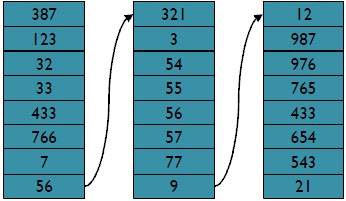
\includegraphics[width=6cm, height=4cm]{Imagenes/Archivo 3.jpg}
        \caption{Lista Enlazada Libre}
        \label{f55} 
        \end{center}
    \end{figure}

    La desventaja es que cuando el bloque está por llenarse puede provocar muchas operaciones de I/O al buscar otro bloque, producto de una serie de \textbf{creaciones y eliminaciones de archivos y directorios}.
    
    \item \underline{\textbf{Base de Datos}} \\
    La tecnología digital se ha convertido en un imperativo para todas las empresas. Necesitándose en ocasiones \textbf{automatizar procesos manuales para mejorar su efectividad}, promoviendo la interconectividad (ver Figura ~\ref{f66}) y mejorando la experiencia del usuario, por ejemplo en la adquisición de materia prima y gestión de la producción en general.
    
     \begin{figure}[H]
        \begin{center}
        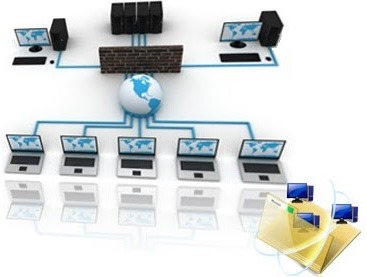
\includegraphics[width=8cm, height=5cm]{Imagenes/Interconec.jpg}
        \caption{Interconectividad Tecnológica}
        \label{f66} 
        \end{center}
    \end{figure}
    
    Cabe resaltar que actualmente, el \textbf{desarrollo de aplicaciones de escritorio y móvil}, se ha convertido en un tema empresarial clave, ya que ayudan a optimizar procesos, reducir costos, mejoran la forma de llegar a los clientes, entre otros beneficios.
    
    Por ello, se desarrollan aplicaciones de escritorio y móvil mediante \textbf{ingeniería de software y listas dinámicas para la gestión y control}. Requiriéndose la administración de una base de datos en específico.
    
    Ante lo mencionado anteriormente se emplean las \underline{estructuras de datos} de listas enlazadas, en particular, porque son estructuras de datos implementadas mediante un grupo de nodos que juntos representan una secuencia, donde cada nodo tiene un dato y una referencia; por ejemplo en la creación de colas, de tipo FIFO,(ver Figura ~\ref{f77}) donde el primer elemento agregado será el primero que saldrá, en órdenes o monitoreo de estado de producción de productos \cite{leon2019desarrollo}.
    
    FIFO, dentro de una base de datos, cuya organizada información o datos estructurados, que normalmente se almacena de forma electrónica en un sistema informático, usando un lenguaje de consulta estructurada (SQL) para escribir y consultar datos, según Vermorel, están destinados a la \underline{optimización cuantitativa} de la cadena de suministro \cite{d}. 
    
     \begin{figure}[H]
        \begin{center}
        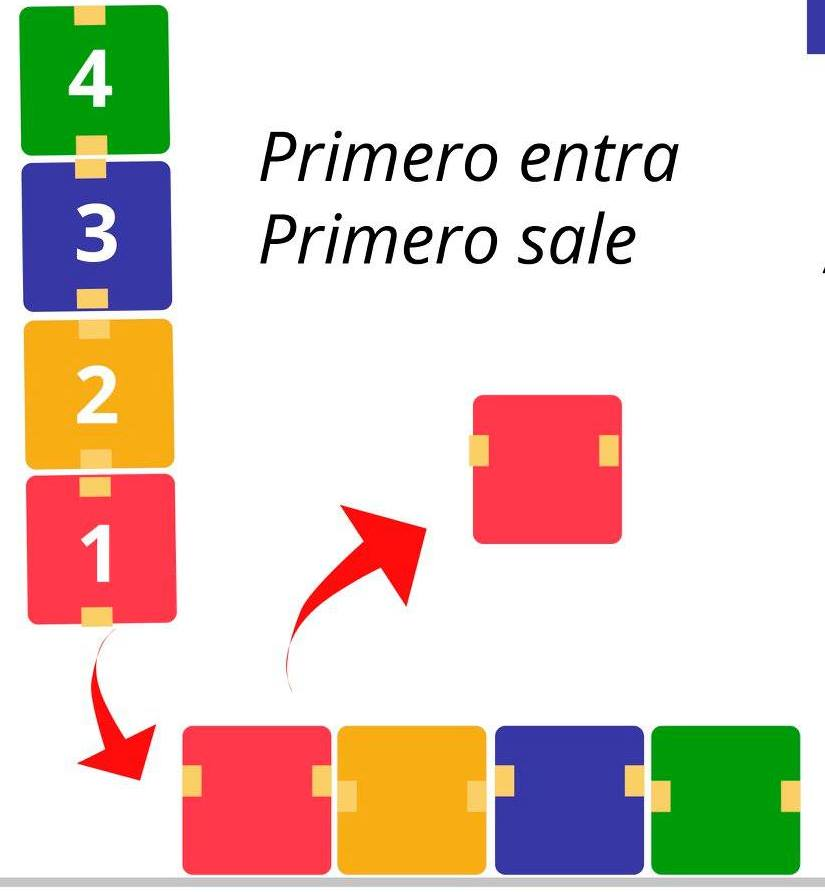
\includegraphics[width=6cm, height=5cm]{Imagenes/FIFO.jpg}
        \caption{Colas - FIFO}
        \label{f77} 
        \end{center}
    \end{figure}
    
    Intuitivamente, dados los niveles actuales de las órdenes de compra en línea, el método FIFO debería devolver, de un modo u otro, \textbf{una composición detallada de la cantidad total}, indicando la antigüedad de cada unidad almacenada. Resulta ser que cada unidad está asociada con una, y solo una, línea de orden de compra.
    
    Este dato estratégico es un tanto sutil, pero da lugar a un método que consiste en calcular, para \textbf{cada línea de orden de compra}, cuántas unidades aún no se vendieron considerando \textbf{los niveles de stock} actuales de los productos dentro de los datos, usando la lectura de archivos: la lista de artículos y la lista de órdenes de compra.
    \end{enumerate}
    
    \section{\textbf{Conclusiones}}
    Es preciso decir que al pasar los años, las nuevas tecnologías han sido muy útiles para organizar, distribuir y almacenar grandes cantidades de datos e información, centrándose siempre en ser más eficientes, dando lugar a las listas enlazadas que son estructuras dinámicas que se utilizan para almacenar datos que están cambiando constantemente.
    
    Por ello, es de suma relevancia en la actualidad, ante el incremento de las bases de datos para la optimización en procesos de productos cuyo sistema formado por un conjunto de datos se almacena en discos permitiendo el acceso directo a ellos.
    
    Finalmente, tanto los archivos y la base de datos hacen uso de listas enlazadas, en el primero se aprovechan todos los bloques del disco, mientras que el segundo menciona a las colas usadas en sistemas informáticos, transportes y operaciones de investigación (entre otros), donde los objetos, personas o eventos son tomados como datos que se almacenan y se guardan mediante colas para su posterior procesamiento.
    
\medskip
\bibliography{Referencia}

\end{document}
